\section{Lezione 10}

\textbf{Generalizzazione}, si applica molto bene agli attori, si parla di \textbf{ereditarietà}.

\begin{center}

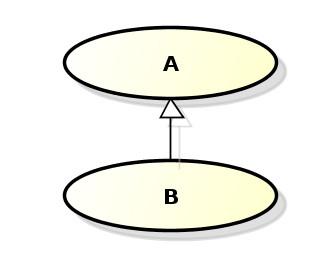
\includegraphics[width=0.75\columnwidth]{img1} % Example image

\end{center}

Se un attore $B$ estende un attore $A$ l'attore $B$ accede a tutte le funzionalità dell'attore $A$ più le sue caratteristiche. Es. l'amministratore è allo stesso tempo un utente normale ma in più ha altri privilegi. La generalizzazione tra casi d'uso è meno usata.

\begin{center}

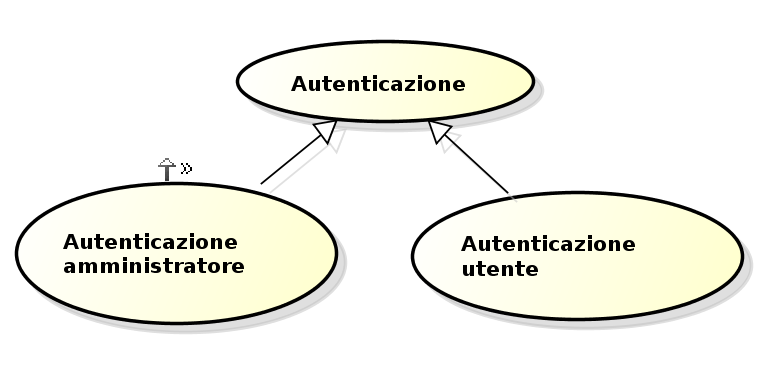
\includegraphics[width=0.75\columnwidth]{img2} % Example image

\end{center}

La generalizzazione fra attori è molto più comune e facile da realizzare:

\begin{center}

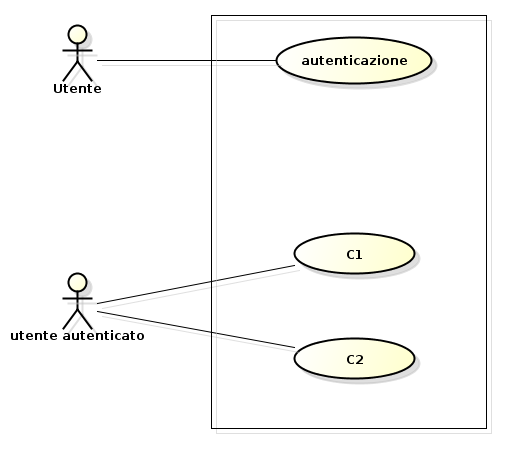
\includegraphics[width=0.75\columnwidth]{img3} % Example image

\end{center}

L'utente non può essere una generalizzazione di un utente autenticato perchè l'utente autenticato non può effettuare autenticazione.

Esempio: l'attore utente può accedere alla funzionalità \textit{autenticazione} del sistema:

\begin{center}

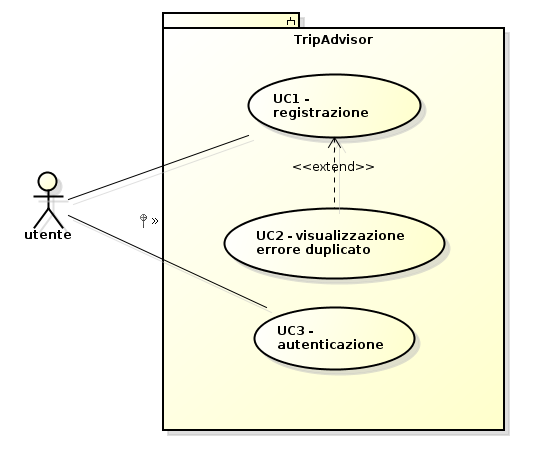
\includegraphics[width=0.75\columnwidth]{img4} % Example image

\end{center}

Scendiamo di dettaglio, meno astratti:

\begin{center}

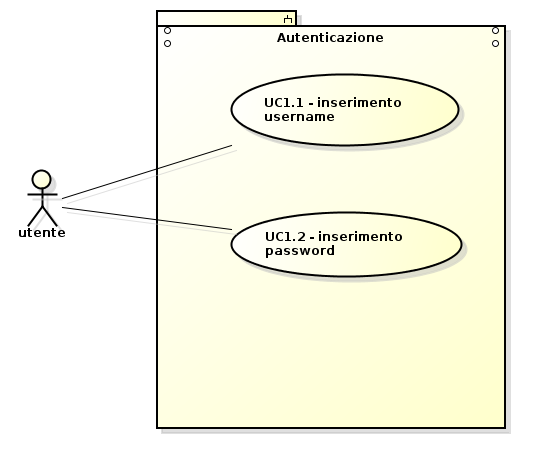
\includegraphics[width=0.75\columnwidth]{img5} % Example image

\end{center}

\textbf{Diagrammi delle classi e degli oggetti}

Il paradigma più utilizzato è il paradigma ad oggetti, perchè modella molto bene la realtà. Ho una lista di requisiti, ora il progettista deve produrre i requisiti e descrivere l'architettura del prodotto, e dovrà descriverla in maniera formale, in modo che i programmatori sviluppino esattamente quello che il progettista ha pensato. Posso in questo modo garantire alcune proprietà. Ho bisogno dunque di un linguaggio per parlare ai programmatori. Una classe è una descrizione di qualcosa e l'oggetto è un'istanza che rispetta questa descrizione. Si passa dalla descrizione a qualcosa di tangibile.

\begin{center}

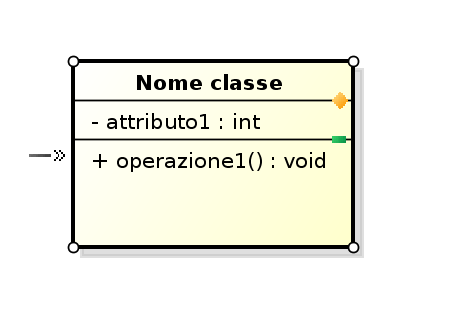
\includegraphics[width=0.75\columnwidth]{img6} % Example image

\end{center}

Modella un concetto ed è indipendente dal linguaggio di programmazione con cui andrò a implementare. La prima cosa che andremo a definire di una classe sono i suoi attributi, che vanno scritti nella parte centrale.

\begin{center}

\texttt{Visibilità nome : tipo [molteplicità] = default [proprietà aggiuntive]}

\end{center}

Questa è la segnatura per la visibilità degli attributi:

\begin{itemize}

	\item \textbf{+}, pubblica;
	\item \textbf{-}, privata;
	\item \textbf{\#}, protetta.

\end{itemize}

\begin{center}

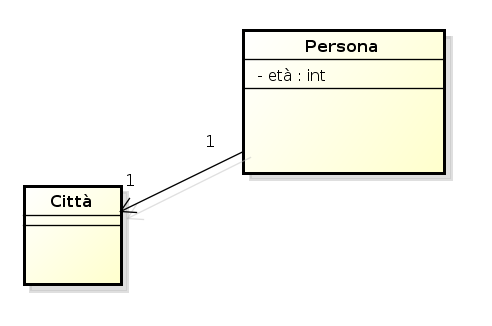
\includegraphics[width=0.75\columnwidth]{img7} % Example image

\end{center}

La molteplicità è 1 perchè una persona ha solo un'età. L'attributo può essere anche espresso come \textbf{associazione} tra due tipi. Questo si fa con una freccia orientata dalla classe che contiene una copia dell'altro tipo. Associazioni senza verso sono bidirezionali. Si utilizzano gli attributi testuali per i tipi primitivi (nella libreria del linguaggio che stiamo utilizzando), mentre si utilizzano le associazioni quando ci si riferisce a due classi del nostro dominio. Se abbiamo molteplicità superiore a 1 significa che abbiamo una collezione (array, liste, ...). Possono esserci delle convenzioni per gli attributi (es. definizione obbligatoria dei metodi \textit{setter} e \textit{getter}. Le proprietà sono gli attributi e le associazioni.

Le operazioni sono ciò che la classe espone verso l'esterno, sono i ``servizi'' della classe.

\begin{center}

\texttt{Visibilità nome (lista-parametri} : tipo-ritorno {proprietà aggiuntive\}}\\
\texttt{Lista-proprietà := direzione nome : tipo = default}

\end{center}

\begin{center}

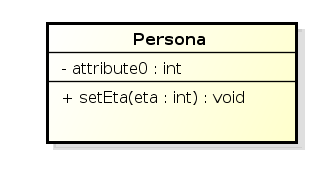
\includegraphics[width=0.75\columnwidth]{img8} % Example image

\end{center}

Le \textbf{query} sono tutte le operazioni che non modificano l'oggetto di invocazione, a differenza dei metodi modificatori. Operazione != metodo, concetto differente in presenza di polimorfismo.\\\textbf{Commenti e note}

\begin{center}

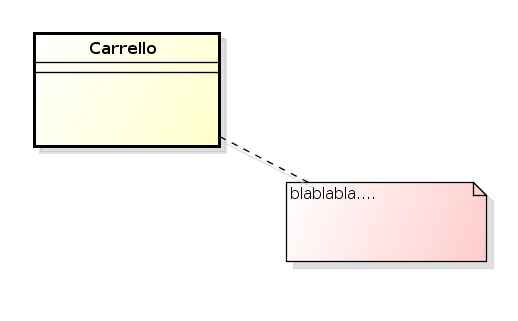
\includegraphics[width=0.75\columnwidth]{img9} % Example image

\end{center}

Un concetto fondamentale è la dipendenza fra due tipi. Una classe $A$ dipende da $B$ se una modifica fatta a $B$ implica una modifica ad $A$. Le dipendenze sono il ``male assoluto'' e vanno minimizzate, perchè le classi devono essere autoconsistenti. Più dipendenze ho e più una modifica può creare \textit{side-effect} su un'altra classe (problemi in fase di manutenzione). Un modo per minimizzare le dipendenze è l'uso di \textbf{interfacce}.

Le dipendenze in UML sono di vario tipo, c'è bisogno di un classificatore, al fine di comprenderla meglio. Questo si inserisce come etichetta nella freccia.

\begin{center}

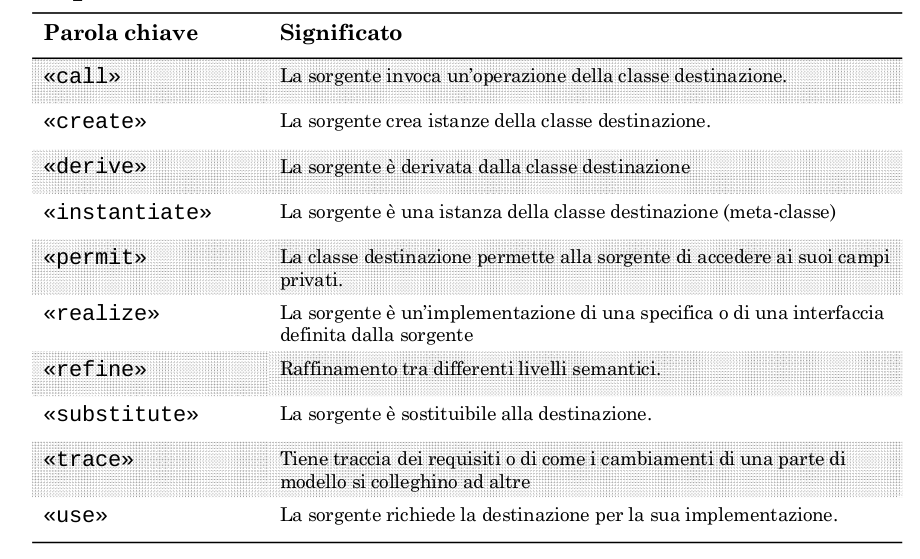
\includegraphics[width=0.75\columnwidth]{img10} % Example image

\end{center}

L'\textbf{aggregazione} e la \textbf{composizione} sono particolari tipi di associazione. L'aggregazione si identifica con la frase ``\textit{parte di...}'', gli aggregati possono essere condivisi. Viene rappresentato con un diamante vuoto. La composizione è come l'aggregazione ma le istanze di un'aggregazione possono appartenere solo ad un aggregato. Solo l'oggetto intero può creare e distruggere le sue parti.

\begin{center}

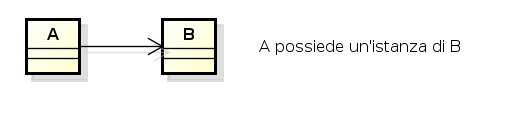
\includegraphics[width=0.75\columnwidth]{img11} % Example image

\end{center}

\begin{center}

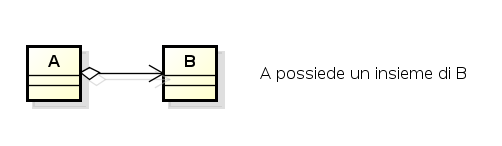
\includegraphics[width=0.75\columnwidth]{img12} % Example image

\end{center}

\begin{center}

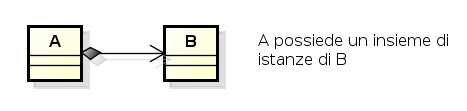
\includegraphics[width=0.75\columnwidth]{img13} % Example image

\end{center}

Può succedere che un'associazione abbia bisogno di essere specificata maggiormente. In questo caso si creano \textbf{classi di associazioni}, che aggiungano attributi ed operazioni alle associazioni. Ma i linguaggi i programmazione non prendono un'implementazione di queste cose.

\begin{center}

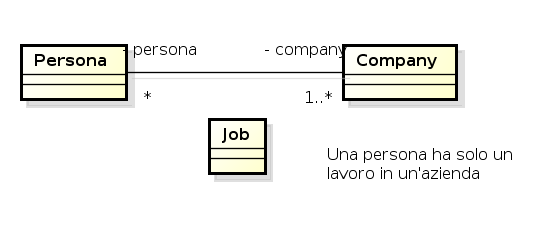
\includegraphics[width=0.75\columnwidth]{img14} % Example image

\end{center}

La \textbf{generalizzazione} è un concetto molto importante, perchè descrive l'ereditarietà, uno dei concetti fondamentali della programmazione a oggetti. $A$ generalizza $B$ se ogni oggetto di $B$ è anche un oggetto di $A$. Sottotipo != Sottoclasse.

\begin{center}

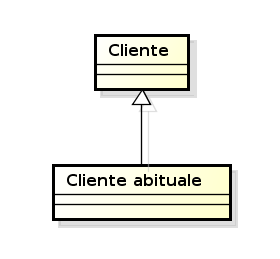
\includegraphics[width=0.75\columnwidth]{img15} % Example image

\end{center}

Per le classi astratte si usa il nome in \textit{corsivo}, non può essere instanziata perché ha delle operazioni che non possiedono l'implementazione, anche se ne può possedere alcune implementate.

Un altro concetto è quello di \textbf{interfaccia}, che non è una classe (al massimo è un tipo) ed è priva di implementazione. Il loro scopo è definire un contratto che le classi che la implementeranno devono assolutamente fornire.

\begin{center}

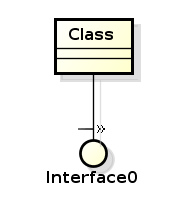
\includegraphics[width=0.75\columnwidth]{img16} % Example image

\end{center}